\documentclass[12pt]{article}
\usepackage[parfill]{parskip}
\usepackage{amsmath}
\usepackage[nottoc,numbib]{tocbibind} % show bib in toc
\usepackage{graphicx}
\usepackage{hyperref}
\linespread{1.5}

\hypersetup{
    colorlinks,
    citecolor=black,
    filecolor=black,
    linkcolor=black,
    urlcolor=black
}

\bibliographystyle{plain}

\title{Perturbation theory and TQSSA}
\author{Oskar Thor\'{e}n}
\date{2015-03-23}

\begin{document}

\nocite{*} % include all references
\maketitle

\begin{abstract}
Perturbation theory has a long history, and recent decades has seen applications
in enzyme kinetics. We start with some basic polynomial examples of perturbation
theory, and then progress to a boundary-value problem in a differential
equation, before we tackle a real application in the form of Total Quasi Steady
State from enzyme kinetics.
\end{abstract}

\clearpage
\tableofcontents
\clearpage

\section{Introduction}

Perturbation theory has its roots in celestial mechanics and
aerodynamics. There are two particularly interesting victories that
perturbation theory has enabled. The first was the discovery of
Neptune, and the second is the theoretical foundation for
aerodynamics.

The promise of perturbation theory is that it allows us to solve a
larger class of problems, for example, in differential equation, than
we could otherwise with analytical methods. It does this by giving us
approximate, but rigorous, solutions. In this article we will guide
the reader from a very simple and familiar example, a quadratic
equation, all the way to a useful research example in system biology:
the total quasi steady state in enzyme kinetics.

The article has been written with the goal that any student with a basic
understanding of calculus, differential equations and linear algebra will be
able to follow along. All the relevant biology and perturbation theory will be
explained as we go along.

\section{A regular perturbation}

We are going to start with one of the simplest non-trivial example imaginable:
a quadratic equation.

\begin{equation}
x^2 - 2x + \epsilon = 0
\end{equation}

We know how to solve this analytically. The roots of the equation are $x_1 = 1 +
\sqrt{1 - \epsilon}$ and $x_2 = 1 - \sqrt{1 - \epsilon}$.

The case we are interested in is the one where $\epsilon$ is very small. In this
case, we can see that setting $\epsilon=0$ produces the roots $x=0$ and $x=2$
respectively. In fact, for any given small $\epsilon$ we notice that solution
changes very little. In that sense it's a very "boring" and predictable problem.

Can we make this observation, that a small change in $\epsilon$ only brings about a small change in the solution, more rigorous? One way is to rewrite the part
of the solution containing $\epsilon$ as a Taylor series. Recall that a Taylor
series for a function $f(x)$ around a point a looks like follows.

\begin{equation}
f(x) = \sum_{n=0}^{\infty} \frac{f^{n}(a)}{n!} (x-a)^n
\end{equation}

The Taylor series for $f(\epsilon) = (1 - \epsilon)^{1/2}$ around 0
(since we assume that \$epsilon$ is very small) is thus:

\begin{equation}
\sqrt{1 - \epsilon} = 1 - \frac{\epsilon}{2} - \frac{\epsilon^2}{8} + O(\epsilon^3)
\end{equation}

Where $O(\epsilon^3)$ is some expression with a term $\epsilon^3$ in
it. If we take the limit of this expression as $\epsilon \to 0$, it's
obvious that our intuition is correct. That is, a small change in
$\epsilon$ only brings about a small change in the solution. We get:

\begin{align}
x_1 &= \frac{\epsilon}{2} + \frac{\epsilon^2}{8} + O(\epsilon^3), \\
x_2 &= 2 - \frac{\epsilon}{2} - \frac{\epsilon^2}{8} + O(\epsilon^3)
\end{align}

What is the point of all this? We said in the beginning that perturbation theory
allows us to solve a larger class of problems, but what we have done so far
hasn't given any indication of that being true. After all, we already have an
analytical formula for the quadratic equation.

Let's start over, but this time let's assume we don't have the quadratic formula
at our disposal. We will outline a method which would allow us to get arbitrarly
good approximations for polynomials of any degree.

Let's assume the solution of (1) in terms of x can be expressed in the
form of a power series of $\epsilon$.

\begin{equation}
\sum_0^{\infty} a_k \epsilon^k = a_0 + a_1 \epsilon + a_2 \epsilon^2 + ...
\end{equation}

We will now insert this power series into (1), and then expand that expression
in terms of powers of $\epsilon$. We only have to do this for the first few
terms of the power series to get a decent approximation. If we want to we can
always add more terms and get a more accurate approximation.

\begin{equation}
(a_0 + a_1 \epsilon + a_2 \epsilon^2 + ...)^2 - 2(a_0 + a_1 \epsilon + a_2
\epsilon^2 + ...) + \epsilon = 0
\end{equation}

We expand the expression using Big-Oh algebra. For example, for the
first term, we get: $(a_0 + a_1 \epsilon + a_2 \epsilon^2)^2 = a_0^2 +
2 a_0 a_1 \epsilon + (a_1^2 + 2 a_0 a_2) \epsilon^2 + O(\epsilon^3)$.

The whole expression becomes the following:

\begin{equation}
a_0^2 - 2 a_0 + (2 a_0 a_1 - 2 a_1 + 1)\epsilon + (a_1^2 + 2 a_0 a_2 - 2 a_2)
\epsilon^2 = O(\epsilon^3), \epsilon \to 0
\end{equation}

Now we turn the problem of determining the coefficients $a_0$, $a_1$ etc. Since
$\epsilon$ is a variable here rather than a parameter, we see that the
coefficients before each power of $\epsilon$ separately all have to be equal to
zero. We thus get the following system of equations for solving the coefficients.

\begin{align}
a_0^2 - 2 a_0 &=0, \\
2 a_0 a_1 - 2 a_1 + 1 &= 0, \\
a_1^2 + 2 a_0 a_2 - 2 a_2 &= 0
\end{align}

Solving these equations in turn gives us, starting with the first
equation, $a_0 = 0$ or $a_0 = 2$. For $a_0 = 0$ we have $a_1 =
\frac{1}{2}$ and $a_2 = \frac{1}{8}$. For $a_0 = 2$ we have $a_1 = -
\frac{1}{2}$ and $a_2 = - \frac{1}{8}$.

We said at the beginning that we assume the solution is on the form of
a power series of $\epsilon$. We have two options for the coefficients
of this power series, and these corresponds to the two approximate
solutions of the original equation. From the above and (6) we get:

\begin{align}
x_1 &= \frac{1}{2} \epsilon + \frac{1}{8} \epsilon^2 + O(\epsilon^3), \\
x_2 &= 2 - \frac{1}{2} \epsilon - \frac{1}{8} \epsilon^2 + O(\epsilon^3)
\end{align}

This is exactly the same as our previous solutions in (4) and (5),
without the use of the quadratica formula. We have thus found a
general method for finding approximate solutions to polynomials of any
degree with a small parameter $\epsilon$.

\section{A singular perturbation}

In the last section we dealt with a so called regular perturbation problem. In this section
we will deal with a singular perturbation problem. What is the difference? In a
singular perturbation problem, the small $\epsilon$ \textit{matters} for the
solution. In general, singular problems are interesting precisely
because their solutions can change significantly with just a small change in
circumstances.

As before, we will use a quadratic equation to illustrate how this works.

\begin{equation}
\epsilon x^2 - 2 x + 1 = 0
\end{equation}

As before, we take $\epsilon$ to be a very small number. This equation has the
following solutions.

\begin{align}
x_1 &= \frac{1 + \sqrt{1 - \epsilon}}{\epsilon}, \\
x_2 &= \frac{1 - \sqrt{1 - \epsilon}}{\epsilon}.
\end{align}

The first thing we notice is that even though $\epsilon$ is very small, we can't
set it to zero. If we were to do it in (14), we would only get a one degree
polynomial. The fact that we are losing solutions is a qualitative change, and
is indicative that we are dealing with a singular perturbation problem.

Let's try using the same method as we did before. We assume x can be
expressed in the form of a power series of $\epsilon$. Inserting this
in our equation gives us the following.

\begin{equation}
\epsilon (a_0 + a_1 \epsilon + a_2 \epsilon^2)^2 - 2(a_0 + \epsilon a_1 +
a_2 \epsilon^2) + 1 = 0
\end{equation}

which gets expanded into.

\begin{equation}
(- 2 a_0 + 1) + (a_0^2 - 2 a_1) \epsilon + (2 a_0 a_1 -2 a_2) \epsilon^2 +
O(\epsilon^3)
\end{equation}

and leads to.

\begin{align}
- 2 a_0 + 1 &= 0, \\
a_0^2 - 2 a_1 &= 0, \\
2 a_0 a_1 -2 a_2 &= 0
\end{align}

$a_0 = \frac{1}{2}$, $a_1=\frac{1}{8}$, $a_2= \frac{1}{64}$, but this gives us
only one of the roots, $x_1$.

\begin{equation}
x_1 = \frac{1}{2} + \frac{1}{8} \epsilon + O(\epsilon^2)
\end{equation}

By the Fundamental Theorem of Algebra, we would expect to see two solutions.
What happened to the other root? We missed it because it's not on the form of
a perturbation series. So what do we do?

The key here is that we can do a change in variable to turn the problem into a
regular perturbation problem.

\begin{equation}
x(\epsilon) = \frac{y(\epsilon)}{\delta(\epsilon)}
\end{equation}

Here we are treating $x$ as a function, $y(\epsilon)$ is $O(1)$ and we want to
determine the re-scaling factor function $\delta(\epsilon)$. Our original
equation becomes

\begin{equation}
\frac{\epsilon}{\delta^2} y^2 - \frac{2}{\delta} y + 1 = 0
\end{equation}

Our goal is to simplify this equation. We do this by dropping relatively
insignificant terms. As we have seen, it turns out that the first term in the
equation is not insignificant, so we have to leave it in. Is there some other
term that we, to a first approximation, can drop?

All the three terms in the above equation have some order of magnitude. The method
of dominant balance tells us to look for pairs that balance, where balance means
they are of the same order of magnitude. We have already determined that the
first term can't be dropped, so we have two options:

\textbf{Case 1.} $\frac{\epsilon}{\delta^2} y^2$ balances 1, with $\frac{2}{\delta}$
being relatively insignificant.

$\frac{\epsilon}{\delta^2} = 1 \implies \delta = \epsilon^{\frac{1}{2}}$. But
then $\frac{2}{\delta} = \frac{2}{\sqrt{\epsilon}}$ which isn't small as
$\epsilon \to 0$.

\textbf{Case 2.} $\frac{\epsilon}{\delta^2} y^2$ balance $\frac{2}{\delta} y$,
with 1 being relatively insignificant.

This means $\frac{\epsilon}{\delta^2} = \frac{1}{\delta}$ which implies that
$\delta = \epsilon$. This seems correct as both expressions are
$O(\frac{1}{e})$, and 1 is relatively small compared to that when $\epsilon \to
0$. We have

\begin{align}
P(x) = \epsilon x^2 - 2x + 1, \\
\epsilon P\Big(\frac{y}{\epsilon}\Big) = y^2 - 2 y + \epsilon
\end{align}

Where the last part is exactly the same as our regular perturbation problem.
Like before, this gives us

\begin{align}
y_1 &= \frac{1}{2} \epsilon + \frac{1}{8} \epsilon^2 + O(\epsilon^3), \\
y_2 &= 2 - \frac{1}{2} \epsilon - \frac{1}{8} \epsilon^2 + O(\epsilon^3)
\end{align}

which means that

\begin{align}
x_1 &= \frac{1}{2} + \frac{1}{8} \epsilon + O(\epsilon^2), \\
x_2 &= \frac{2}{\epsilon} - \frac{1}{2} + \frac{1}{8} \epsilon + O(\epsilon^2)
\end{align}

The second root is our missing solution, and it corresponds to $x \to \infty$ as
$\epsilon \to 0$. This is the essence of singular perturbation theory - to find
the singular behavior and do a change of variable to turn it into a regular
perturbation problem.

\section{ODE and boundary theory}

Boundary layer theory has its origins in aerodynamics and Prandtl. He
discovered that the way fluids, like air around a plane and water
around some obstacle, flows is almost completely void of viscosity, or
stickiness, except for in a very thin region near the boundary of the
plane of the obsacle. This allowed for the separate treatment - one
where viscosity can be discarded, and one where it matters a lot - of
what would back then be one single complex problem, which simplified
matters greatly.

We will now give a basic example of this in the form of a boundary
value problem with differential equations. We will again look at a
problem which we could solve explicitly, but instead use perturbation
theory to analyze. In a boundary value problem, we have two boundary
value conditions and, in a first approximation, they can't both be
satisfied at the same time. The strategy we use is to split the
problem in two - one where we are in a very thin region at $t=0$
(where we have a boundary condition), the so called inner region, and
one where we are in an outer region, which is everywhere else. This
strategy is generalizable to multiple layers.

We start by looking for the outer solution, then the inner solution,
then we match them together into one unified solution.

\subsection{Outer solution}

We are now going to look at a differential equation.

\begin{equation}
\epsilon y'' + 2 y' + y, y(0)=0, y(1)=1, 0 < x < 1
\end{equation}

If we naively set $\epsilon = 0$ we see that the resulting equation $2 y' + y$
has the general solution $C e^{- \frac{1}{2}x}$. This can't satisfy both
boundary conditions at once. If it satisfies $y(0)=0$ we have $y=0$ as the only
solution, and if it satisfies $y(1)=1$ we have

\begin{equation}
y_O=e^{\frac{1}{2} (1 - x)}
\end{equation}

We are going to assume this is a good approximation somewhere. We are also going
to assume this is valid for the $y(1)=1$ boundary condition. We call this out
outer solution.

Like the example in the last section, we missed something when we set $\epsilon
= 0$. We have found one of the two solutions and now we want to the find the
other one with the help of pairwise balancing.

\subsection{Inner solution}

We are assuming the boundary layer is near 0, and that it has a thickness
$\delta(\epsilon)$. We introduce a re-scaling variable

\begin{equation}
\overline{x} = \frac{x}{\delta}
\end{equation}

Having two scales like this is typical for singular perturbation problems. Our
original equation (31) becomes

\begin{equation}
\frac{\epsilon}{\delta^2} \frac{d^2y}{d\overline{x}^2} + \frac{2}{\delta}
\frac{dy}{d\overline{x}} + y = 0
\end{equation}

We now do pairwise balancing. We have the following orders of
magnitude

\begin{equation}
\frac{\epsilon}{\delta^2}, \frac{1}{\delta}, 1
\end{equation}

We must have $\frac{\epsilon}{\delta^2}$ present, so the question is if it
balance one of the other terms with one being insignificant, and if so, which one
is insignificant. There are two cases.

\textbf{Case 1}
\begin{equation}
\frac{\epsilon}{\delta^2} ~ 1 \implies \delta = \epsilon^{\frac{1}{2}},
\end{equation}

but then $\frac{1}{\delta}$ is big compared to 1.

\textbf{Case 2}
\begin{equation}
\frac{\epsilon}{\delta^2} ~ \frac{1}{\delta} \implies \delta = \epsilon,
\end{equation}

in which case 1 is indeed insignificant.

We have, multiplying by $\epsilon$, the inner equation:

\begin{equation}
\frac{\delta^2 y}{\delta \overline{x}^2} + 2 \frac{dy}{d\overline{x}} + \epsilon
y = 0
\end{equation}

To a first approximation we can neglect the last term

\begin{equation}
\frac{\delta^2 y}{\delta \overline{x}^2} + 2 \frac{dy}{d\overline{x}} = 0
\end{equation}

Together with the other initial condition $y(0)=0$ we get the general inner
solution, valid in a region of thickness $\epsilon$ close to $x=0$

\begin{equation}
y_I = C(1 - e^{-2\overline{x}})
\end{equation}

We now have an outer and inner solution, and we turn to matching these to
determine the constant $C$.

\subsection{Matching}

The idea behind matching is that there is some edge or region between the inner
and outer solution. A region where both solutions are valid approximations.

If we imagine a particle tracing the x-axis rightward, as we exit the boundary
layer, i.e. as $\overline{x} \to \infty$, the value of $y_I$ should be equal to
the value of $y_O$ as $x \to 0$, that is

\begin{equation}
\lim_{\overline{x} \to \infty} y_I = \lim_{x\to 0+} y_O \iff 
\lim_{\overline{x} \to \infty} C(1 - e^{-2\overline{x}}) = \lim_{x \to 0+} e^{\frac{1}{2}(1-x)}
\end{equation}

This is called a \textit{matching condition}. The right-hand side is
$e^{\frac{1}{2}}$, and thus the left-hand side gives us that $C =
e^{\frac{1}{2}}$.

\subsection{Uniform approximation}

We now have two separate approximations. We would like to have one single
approximation that is valid everywhere. We do this by adding the two
approximations together and removing their common part.

\begin{equation}
y_U = y_o(x) + y_I(\frac{x}{\delta}) - e^{\frac{1}{2}}
\end{equation}

The common part comes from the matching condition in the previous section. In
the inner region the other terms are negliable, and vice versa in the outer
region.

\begin{align}
y_U &= e^{\frac{1}{2}(1-x)} e^{\frac{1}{2}}(1 - e^{\frac{-2x}{\epsilon}}) -
e^{\frac{1}{2}} \\
    &=  e^{\frac{1}{2}}(e^{\frac{-x}{2}} - e^{\frac{-2x}{\epsilon}})
\end{align}

Which is our uniform approximation for the whole solutions.

We can compare this to the exact solution and see that it is indeed a good
approximation.

\subsection{Comparison with exact solution}

We saw in the previous section what a good approximation to the
solution is. Our original equation (31) can however be solved exactly,
so let's do that.

The characteristic polynomial $\epsilon r^2 +2r + 1 = 0$ has the solutions
$\frac{-1 \pm \sqrt{1-\epsilon}}{\epsilon}$. We have:

\begin{equation}
y_{\epsilon}(x)=c_1 e^{\frac{-1 + \sqrt{1-\epsilon}}{\epsilon} x} + c_2
e^{\frac{-1 - \sqrt{1-\epsilon}}{\epsilon} x}
\end{equation}

With the help of the boundary conditions $y(0)=0, y(1)=1$ we see that

\begin{equation}
  c2 = - c1 = - \frac{1}{e^{\frac{-1 + \sqrt{1-\epsilon}}{\epsilon}}
    - e^{\frac{-1 - \sqrt{1-\epsilon}}{\epsilon}}}
\end{equation}

We use a Taylor expansion as before and define $\alpha_1$ and $\alpha_2$ as follows:

\begin{align}
  \alpha_1 &= \frac{1 - \sqrt{1-\epsilon}}{\epsilon} = \frac{1}{2} + O(\epsilon) \\
  \alpha_2 &= 1+ \sqrt{1-\epsilon} = 2 + O(\epsilon)
\end{align}

We can then express the solution as follows:

\begin{equation}
  y_{\epsilon}(x) = \frac{1}{e^{-\alpha_1(\epsilon)} - e^{\frac{-\alpha_2(\epsilon)}{\epsilon}}} \Big(e^{-\alpha_1(\epsilon)x} - e^{\frac{-\alpha_2(\epsilon)x}{\epsilon}}\Big)
\end{equation}

There are two terms in this solution. As $\epsilon \to 0+$, for fixed
$x \in (0,1)$, all the expression involving a division with $\epsilon$
disappears. The solution becomes:

\begin{equation}
  y_{\epsilon}(x) \to \frac{e^{\frac{-x}{2}}}{e^{\frac{-1}{2}}} = e^{\frac{1}{2}(1-x)}
\end{equation}

This is exactly the outer solution we got before, satisfying $y(1)=1$
but not $y(0)=0$.

If we instead take (49) and notice that, for arbitrarily small
$\epsilon$, $e^{-\frac{\alpha_2(\epsilon)}/{\epsilon}}$ is 0. The
exact solution is thus (we distinguish between an approximation of the
exact solution, and the outer approximation):

\begin{equation}
y_{\epsilon}(x) \approx e^{\frac{1}{2}}(e^{-\frac{x}{2}} -
  e^{-\frac{2x}{\epsilon}}), \quad 0 < \epsilon \ll 1
\end{equation}

When we graph (50) and (51) for any given $\epsilon$ we see that,
outside of a small region near 0, the outer approximation is indeed a
good approximation.

\begin{figure}[ht!]
\centering
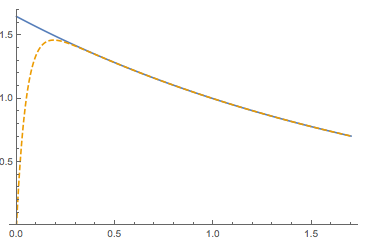
\includegraphics[width=120mm]
{tmp_ode-outer.png}
\caption{The full line is the outer approximation, $\epsilon=0.1$}
\label{overflow}
\end{figure}

Note that the outer approximation starts at $y(0)=e^{\frac{1}{2}}$,
and thus misses the contribution $\epsilon$ has on the solution for
very small x values.

If we were to do the same thing for the inner solution, we would get
the following graph.

\begin{figure}[ht!]
\centering
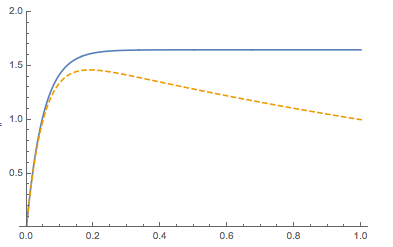
\includegraphics[width=120mm]
{tmp_ode-inner.png}
\caption{The full line is the inner approximation, $\epsilon=0.1$}
\label{overflow}
\end{figure}

Notice the agreement between the exact and inner approximation in a
region close to $x=0$ (which we can move arbitrarily closer by using a
smaller $\epsilon$).

\section{Total Quasi Steady State}

\subsection{A biological problem}

In enzyme kinetics we often come across chemical reactions like

\begin{equation}
E + S \leftarrow_{k_1} \rightarrow_{k_{-1}} C \rightarrow_{k_2} E + P
\end{equation}

This is an enzyme E and substrate S that combine, reversibly, to form a complex
C, which in turn gives us a product and enzyme back. $k_1, k_{-1}, k_2$ are rate
constants. We won't bother with the biological etails too much, but instead look
at how we can analyze the above as a dynamical system.

The \textit{law of mass action} tells us that two molecules A and B forming
complex C, $A+B \rightarrow_k C$ are governed by $\frac{dC}{dt} = kAB$. That is,
the more concentration of A or B we have, the faster they turn into complex C.
This has been experimentally verified by Guldberg and Waage in 1867, and many
times since.

With this law, we can translate our chemical reaction a system of differential
equations.

\begin{align}
\frac{dE}{dt} &= -k_1(E*S) + k_{-1}C + k_2C, \\
\frac{dS}{dt} &= -k1(E*S) + k_{-1}C, \\
\frac{dC}{dt} &= k_1(E*S) - k_{-1}C - k_2C, \\
\frac{dP}{dt} &= k_2C
\end{align}

In the study of enzyme kinetics, we normally have some initial conditions to help
us out: $S(0) = S_0, E(0) = E_0, C(0)=0, P(0)=0$.

We see immediately that

\begin{equation}
\frac{dE}{dt} + \frac{dC}{dt} = 0
\end{equation}

Together with the initial conditions we get that

\begin{equation}
E + C = E_0
\end{equation}

Which we can use to eliminate E from the equation. This is called a conservation
law.  We also don't care about P, as it doesn't feed back into the other
equations. We are left with

\begin{align}
\frac{dS}{dt} &= -k_1(E_0 - C)S + k_{-1}C, \\
\frac{dC}{dt} &= k_1(E_0 - C)S - k_{-1}C - k_2 C
\end{align}

This is a two-dimensional system, which is much easier to deal with. Can we do
better? It turns out we can.

Very often, in practice, the substrate has a much higher concentration than enzyme. This
means that C can be treated as constant after a short initial period. By
exploiting this fact, we can reduce the system to one equation. This is called
the \textit{Quasi-Steady State approximation}.

Assume that C is constant $\iff \frac{dC}{dt} = 0$ after a short period of time,
then we can could write, as $\frac{dC}{dt}$ can be treated as 0,

\begin{equation}
\frac{dS}{dt} = -k2 C
\end{equation}

with

\begin{equation}
C = \frac{E_0 S}{K_m +S}
\end{equation}

where $K_m = \frac{k_{-1} + k_2}{k_1}$ is the so called {Michaelis-Menten
constant}.

\begin{equation}
\frac{dS}{dt} = \frac{-k_2 E_0 S}{K_M + S}
\end{equation}

together with $S(0) = S_0$ as initial condition is what is normally considered
the QSSA, valid after some short amount of time has passed.

We can justify this with a procedure similar to the previous section, as done by
for example Lin and Segel \cite{lin1974mathematics}. Instead we are going to
look at a slight variation of this, namely what happens when the amount of
substrate isn't much bigger than the amount of enzymes. This is the
\textit{Total Quasi Steady State assumption}, discovered by Borghans and Segel
1996 \cite{borghans1996extending}.

\subsection{TQSSA}

The basic idea behind TQSSA is to perform a change of variable

\begin{equation}
\overline{S} = S + C
\end{equation}

This change of variable makes the approximation valid for more parameters. We
get the following system of equations from (52), (53) and (57)

\begin{align}
\frac{d\overline{S}}{dt} &= - k_2 C, \\
\frac{dC}{dt} &= k_1(E_0-C)(\overline{S}-C)-(k_{-1}+ k_2) C
\end{align}

With initial conditions $\overline{S}(0)=S_0, C(0)=0$, these are the rate
equations for the TQSSA.

\begin{figure}[ht!]
\centering
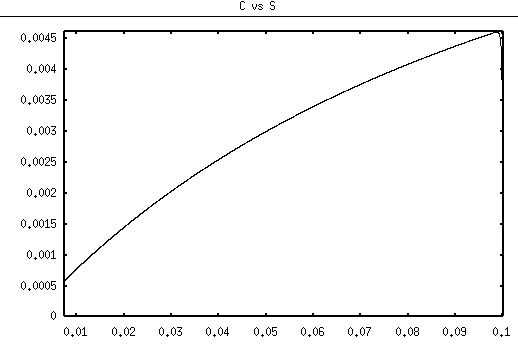
\includegraphics[width=120mm]
{tqssa-phase-plane-b.png}
\caption{TQSSA phase plane. Initial state is $\overline{S}(0)=0.1,
  C(0)=0$. $E=0.01, k_1=10, k={-1}=1, k_2=0.1$.}
\label{overflow}
\end{figure}

We get some intuition of the behavior by inspecting the phase plane of
the above equations. With the help of XPP (see appendix for the source
code used), we can numerically simulate the system, as seen in figure
1. There are two things to note: (1) the steady state is at (0,0) (not
shown in graph due to numerical rounding error) and (2) from the initial
condition there's a rapid increase of concentration in complexity C,
after which it slowly decrease (quasi-steady state) until it reached
steady state.

\subsection{Timescales}

To analyze the problem rigorously using perturbation theory, we need
to find an expression that estimates these two time scales that the
system is operating with, $t_c$ for the fast initial period and
$t_{\overline{s}}$ for the slow quasi-steady state period.

To get the fast time scale, we can estimate S as $S_0$ since in that
time period the substrate concentration won't change much. We just
care about rough orders of magnitudes for the timescales. From (60) we
get:

\begin{equation}
  \frac{dC}{dt} = k_1E_0 S_0 - (k_1 S_0 + k_{-1} + k_2)C
\end{equation}

With the help of initial condition $C(0)=0$, we get the solution:
$C(0)=0$):

\begin{equation}
  C(t) = A(1 -  e^{\lambda x}), \quad
  \lambda = (-S_0 k_1 + k_{-1} + k_2), \quad
  A =\frac{k1 E_0 S_0}{S_0 k1 + k_{-1} + k_2}
\end{equation}

The timescale here is $t_c = \lambda^{-1}$, which we can rewrite as:

\begin{equation}
  t_c = \frac{1}{k_1(S_0+K_M)}
\end{equation}

To get the other time scale we first use that $dC/dt = 0$ after some
period of time, which is the time scale we care about. We then use
(61) and (62) as before to get (63):

\begin{equation}
  \frac{dS}{dt} = -\frac{k_2 E_0 S}{K_M + S}
\end{equation}

We now get $t_s$ with the help of an estimation technique by Segel
\cite{segel1984modeling} that tells us to take $S_0$ divided by the
maximum of $|dS/dt|$ using $S_S0$ in the previous equation. This gives
us:

\begin{align}
  t_s &= \frac{S_0}{|dS/dt|_{max}}, \\
      &= \frac{K_M + S_0}{k_2 E_0}
\end{align}

So far we have only derived timescales for the normal QSSA. To get the
timescales for TQSSA, Borghans et al. use the rewrite $\overline{S} =
S + C$. By doing so, and assuming $dC/dt=0$ as before, the $dC/dt$
equation gets a quadratic term, $C^2$:

\begin{equation}
  C^2 - (E_0 + K_M + \overline{S})C + E_0 \overline{S} = 0
\end{equation}

They then use a so called two-point Pad\'{e} approximant to simplify
the resulting expression. (Alternatively it can be shown that
neglecting the $C^2$ term gives a good approximation, but this is
outside the scope of this article.). The Pad\'{e} approximant of the
above equation is:

\begin{equation}
  C = \frac{E_0 \overline{S}}{E_0 + K_M + \overline{S}}
\end{equation}


Eventually we end up with these two slightly modified time-scales:

\begin{align}
t_c &= \frac{1}{k_1(E_0+S_0+K_M)}, \\
t_{\overline{s}} &= \frac{E_0+S_0+K_m}{k_2+E_0}
\end{align}

$K_M = \frac{k_{-1}+k_2}{k_1}$ as before. We will now analyze this
like we did in the last section. But first, we have to scale the
system using our newly discovered timescales.

\subsection{Scaling}

Lin and Segel defines Scaling as follows:

\textit{Scaling amounts to nondimensionalizing so that relative magnitude of
each term is indicated by a dimensionless factor preceding that term}
\cite{lin1974mathematics}.

We will now introduce scaled, dimensionless variables. We get these variables by
dividing with their respective scales. We have the two time variables:

\begin{align}
t_f &= \frac{t}{t_c}, \\
t_s &= \frac{t}{t_{\overline{S}}}
\end{align}

$t_f$ is the fast time scale, and $t_s$ the slow one. We also scale C and
$\overline{S}$ by their maximum:

\begin{align}
c &= \frac{C}{C_0}, \\
s &= \frac{\overline{S}}{S_0}
\end{align}

$S_0$ is max since it starts from some constant and then turns into
complex, as we saw before. Borghans et al. derive C's max (or an upper
limit for it), $C_0$ by using the Pad\'{e} approximation in (74) and
$S=S_0$:

\begin{equation}
C_0 = \frac{E_0 S_0}{E_0 + S_0 + K_m}
\end{equation}

\subsection{Outer solution}

We now have a mathematical formulation of the problem and we just need a small
parameter $\epsilon$ to begin looking for the outer solution, where the complex
changes slowly.

A necessary condition for TQSSA to hold is $0 < \epsilon \ll 1$

\begin{equation}
\epsilon = \frac{t_f}{t_s}
\end{equation}

This comes from Borghans. \textit{Assuming} $t_f \ll t_s$ we then get, for the
outer region.

Using c and $t_s$ we get, using the procedure used by Khoo and Heglund
\cite{khoo2008total},

\begin{equation}
\frac{dC}{dt_s} = \frac{t_{\overline{S}}}{c_0} k_1 [E_0 S_0 s - (E_0 + S_0 s +
K_M) C_0 c + (c c_0)^2]
\end{equation}

Recall that

\begin{equation}
\epsilon = \frac{t_f}{t_s} = \frac{k_2 E_0}{k_1(E_0+S_0+K_m)^2}
\end{equation}

so we can rewrite the above as

\begin{equation}
... = \frac{1}{\epsilon} (s - \frac{E_0+S_0 s + k_m}{E_0 + S_0+ K_M}C + \gamma^2
c)
\end{equation}

\begin{equation}
\gamma = \frac{E_0 S_0}{(S_0 + K_m + E_0)^2}
\end{equation}

TODO: Check algebra and lower case c, s.

TODO: This reasoning is wrong, It's due to Tikhonov theorem (C433)

As $\epsilon \to 0, \frac{1}{\epsilon} \to \infty$, but C(0) = 0 so

\begin{equation}
s - \frac{E_0 + S_0 s + K_m}{E_0 + S_0 + K_M}C + \gamma c^2 = 0
\end{equation}

TODO: What is it? How do they work? Take for granted or explain?

By using Pade approximants we can get an approximation for the outer
solution

\begin{equation}
c_0  = \frac{E_0 + S_0 + K_m}{E_0 + S_0 s + K_m} s
\end{equation}

This is the outer solution. If we substitute this into s we get an
expression for outer solution of s.

TODO: Check algebra. Mathematica?

\begin{equation}
\frac{ds}{dt_s} = \frac{-E_0 + S_0 + K_m}{E_0 + S_0s + k_m}s, s(0) = 1
\end{equation}

Solving this, we get the outer solution for s, according to Khoo:

TODO: Derive yourself? Same below

\begin{equation}
(E_0 + K_m) ln s_O(t_s) + s_o(s_o(t_s) - 1) + (E_0 + S_0 + K_m) t_s = 0
\end{equation}

\subsection{Inner solution}

TODO: Show intermediate steps. Which ones?

Using the outer time scale to satify the other initial conditions,

\begin{equation}
\frac{dS}{dt_f} = \frac{-k_2 E_0}{k_1(E_0 + S_0 + K_M)^2} c, s(0) = 1
\end{equation}

As $\epsilon \to 0$, the above becomes $\frac{dS}{dt_f} = 0$, i.e constant.

\begin{equation}
s_I = s(0) = 1
\end{equation}

For c:

\begin{equation}
\frac{dc}{dt_f} = 1 - c - \gamma c^2, c(0)=0
\end{equation}

TODO: How solve this? Mathematica?

Khoo et al. finds that the solution is

\begin{equation}
c_I = \frac{2[exp(\sqrt{4\gamma-1}t_f)-1]}{(1-\sqrt{1-4\gamma}
exp(\sqrt{4\gamma-1}t_f) - (1+\sqrt{1-4\gamma}}
\end{equation}

where c(0)=0 holds.

TODO: Check this.

\subsection{Matching}

As before, we are looking for a common limit, and our matching condition as
$\epsilon \to 0, t_f \to \infty, t_s \to 0$ is

\begin{equation}
\lim \epsilon 0 [y_o(t_s)|t_s=0] = \lim \epsilon \to 0[y_I(t_f)|t_f=\infty]
\end{equation}

For s:

\begin{equation}
\lim \epsilon 0 [y_o(t_s)|t_s=0] = \lim \epsilon \to 0[y_I(t_f)|t_f=\infty] = 1
\end{equation}

For c:

TODO: Perform this limit check, help from Mathematica? Can I find by hand? Khoo
finds

\begin{equation}
... = \approx 2(1+\sqrt{1-4\gamma})^{-1}
\end{equation}

\subsection{Uniform approximation}

Like before, we take the common part and subtract the difference.

\begin{align}
s_u &= s_O + s_I - 1 = s_O, \\
c_u &= c_O + c_I - 2(1 + \sqrt{1-4\gamma})^{-1}
\end{align}

TODO: Phase plane / numerical? Same as before. But compared to what?

\section{Appendix}

\subsection{TQSSA XPP code}

\begin{verbatim}
# tqssa.ode
# k = k1, l=k_1, m=k2
#
s'=-m*c
c'=k*(e-c)*(s-c)-(l+m)*c
par e=0.01, k=10, l=1, m=0.1
init s=0.1, c=0
@xp=s, yp=c
# xlo=0, ylo=0, xhi=1, yhi=1
@ total=400
@ nmesh=51
done
\end{verbatim}

To reproduce, download XPP and load the above code. Press "V 2" and
choose S on the x-axis for the phase plane, press "I G" to simulate
from the initial conditions, then "W F" to fit the resulting graph to
the window. If we press "S G" we get a confirmation that there's a
steady state at at (0,0) to a rounding error becuase of numerical
errors, and that it is stable. For more information, consult the
official XPP manual available online.

\subsection{Mathematica code}

\begin{verbatim}
f[x_] := E^((1/2) (1 - x)) (* outer approx *)
g[x_] := E^(1/2) (E^(-x/2) - E^(-2 x/err)) (* exact *)
h[x_] := E^(1/2) * (1 - E^(-2*x/err)) (* inner approx *)
err = 0.1

Plot[{f[x], g[x]}, {x, 0, 1.7}, PlotRange -> {0, 1.7}, PlotStyle ->
 {Dashing, Directive[Dashed], Directive[Thick]}]

Plot[{h[x], g[x]}, {x, 0, 1}, PlotRange -> {0, 2}, 
 PlotStyle -> {Dashing, Directive[Dashed], Directive[Thick]}]
\end{verbatim}

\bibliography{references}

\end{document}
